\chapter{Low Cost Coordination}

Millions of sensors, mobile applications, users, and machines now
continuously generate billions of events.
%
These events are processed by streaming
engines~\cite{spark-streaming, trill} and ingested and aggregated
by state management systems (Figure~\ref{fig:pipeline}).
%
Real-time queries are issued against this ingested data to train and
update models for prediction, to analyze user behavior, or to generate
device crash reports, etc.
%
Hence, these state management systems are a focal point for massive numbers of
events and queries over aggregated information about them.

\begin{figure}[t]
\centering
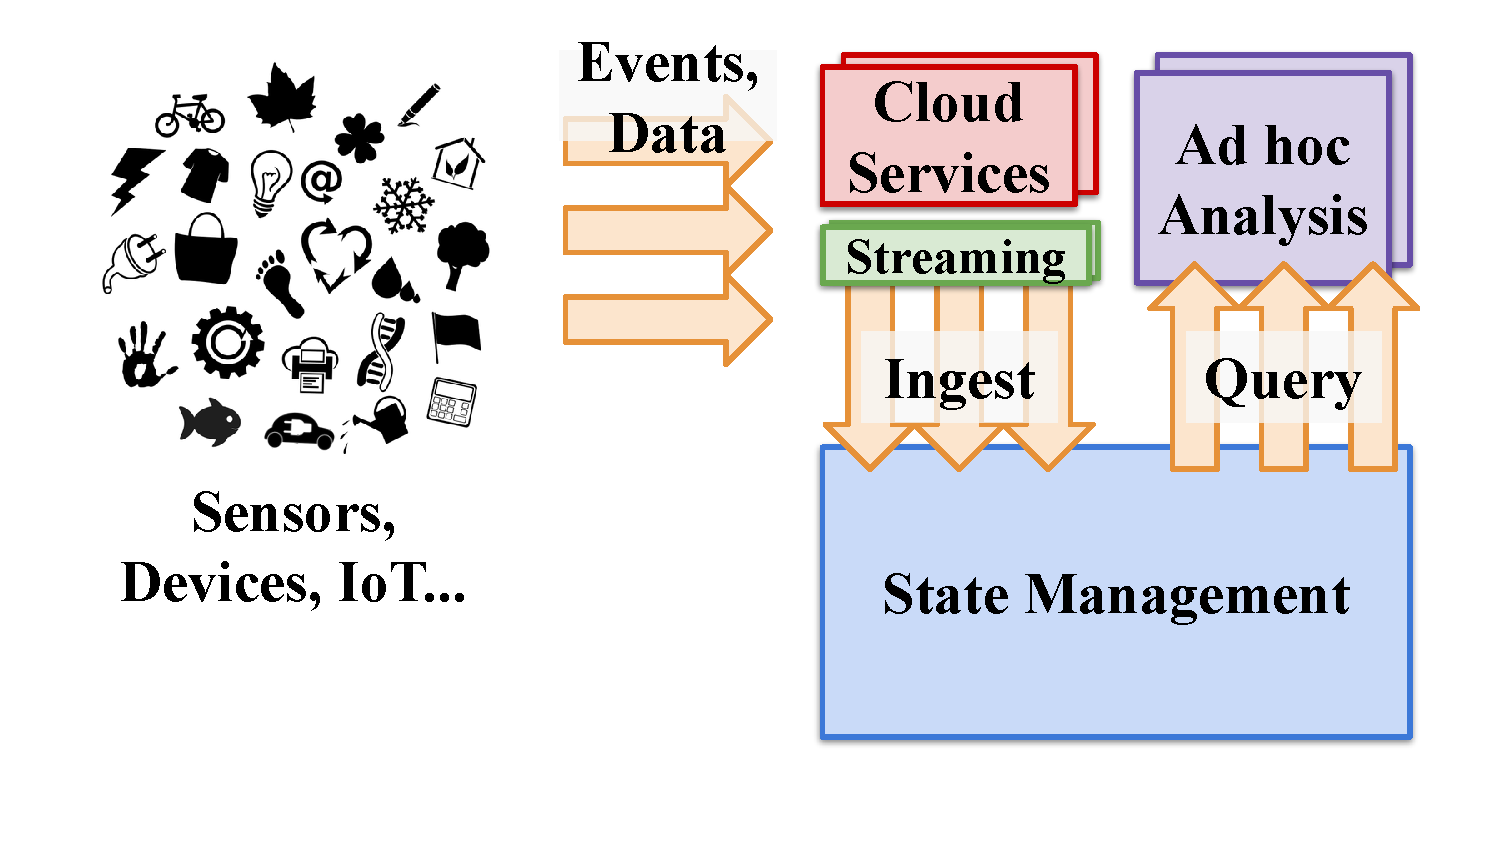
\includegraphics[width=0.93\columnwidth]{figures/pipeline.pdf}
\caption{
A typical data processing pipeline. Services receive and
process raw events and data. A state management system ingests processed
events and data, and serves offline queries against them.}
\label{fig:pipeline}
\end{figure}


Recently, this has led to specialized key-value stores (KVSs) that can
ingest and index these events at high rates -- 100 million operations
(Mops) per second (s) per machine -- by
exploiting many-core hardware~\cite{faster,anna}.
%
These systems are efficient if events are generated on the same machine as
the KVS, but, in practice, events need to be aggregated from a wide
and distributed set of data sources.
%
Hence, fast indexing schemes alone only solve part of the problem.
%
To be practical and cost-effective, a complete system for aggregating these
events must ingest events over the network, must scale across machines as
well as cores, and must be elastic (by provisioning and reconfiguring over
inexpensive cloud resources as workloads change).

The only existing KVSs that provide similar
performance~\cite{mica,flexnic,floem,kvdirect} rely on application-specific
hardware acceleration, making them impossible to deploy on today's cloud
platforms.
%
Furthermore, these systems only store data in DRAM, and they do not scale across
machines; adding support to do so without cutting into normal-case performance
is not straightforward.
%
For example, many of them statically partition records across cores to
eliminate cross-core synchronization.
%
This optimizes normal-case performance, but it makes concurrent
operations like migration and scale out impossible; transferring record data
and ownership between machines and cores requires a stop-the-world approach
due to these systems' lack of fine-grained synchronization.

Achieving this level of performance while fulfilling all of these
requirements on commodity cloud platforms requires solving two key challenges
simultaneously.
%
First, workloads change over time and cloud VMs fail, so systems must tolerate
failure and reconfiguration.
%
Doing this without hurting normal-case performance at 100~Mops/s is hard, since
even a single extra server-side cache miss to check key ownership or
reconfiguration status would cut throughput by tens-of-millions of operations
per second.
%
Second, the high CPU cost of processing incoming network
packets easily dominates in these workloads,
especially since, historically, cloud networking stacks have not been designed
for high data rates and high efficiency.
%
However, this is changing; by careful design of each server's data path, cloud
applications can exploit transparent hardware acceleration and offloading
offered by cloud providers to process more than 100~Mops/s per cloud virtual
machine (VM).

\emph{Shadowfax} is a new distributed KVS that transparently
spans DRAM, SSDs, and cloud blob storage while serving 130~Mops/s/VM over
commodity Azure VMs~\cite{azure} using conventional Linux TCP.
%
Beyond high single-VM performance, its unique approach to
distributed reconfiguration avoids any server-side key ownership checks
and any cross-core coordination during
normal operation and data migration both in its indexing and network interactions.
%
Hence,
it can shift load in 17~s to improve cluster throughput by
10~Mops/s
with little disruption.
%
Compared to the state-of-the-art, it has 8$\times{}$ better throughput (than
Seastar+memcached~\cite{seastar}
(Figure~\ref{fig:seastar})) and scales out 6$\times{}$ faster (than
Rocksteady~\cite{rocksteady}).

\begin{figure}[t]
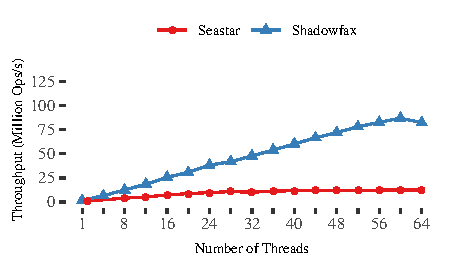
\includegraphics[width=\textwidth]{graphs/seastar.pdf}
\caption{
Shadowfax’s thread scalability. With TCP acceleration enabled,
throughput scales linearly to 87 Mops/s under a uniform distribution. In
comparison, Seastar scales to 10 Mops/sec.
}
\label{fig:seastar}
\end{figure}


Three key pieces of Shadowfax help
eliminate coordination throughout the client- and server-side by eliminating
cross-request and cross-core coordination:
%
\begin{description}
\item[Low-cost Coordination via Global Cuts:]
% All of the major components of Shadowfax including indexing, request
% dispatching, durability, checkpointing/recovery, and migration center
% around a key mechanism: asynchronous \emph{global cuts}~\cite{faster,cpr,scalog}.
%
In contrast to totally-ordered or stop-the-world approaches used by most
systems, cores in Shadowfax avoid stalling to synchronize with one another, even when
triggering complex operations like scale-out, which require
defining clear before/after points in time among concurrent operations.
%
Instead, each core participating in these operations -- both at clients and
servers -- independently decides a point in an \emph{asynchronous global
cut} that defines a boundary between operation sequences in these complex operations.
%
Shadowfax extends asynchronous cuts from cores within one
process~\cite{faster} to servers
and clients in a cluster.
%
This helps coordinate server
and client threads (through partitioned sessions)
in Shadowfax's low-coordination data migration and
reconfiguration protocol.

\item[End-to-end Asynchronous Clients:]
All requests from a client on one machine to Shadowfax are asynchronous with
respect to one another all the way throughout Shadowfax's client- and
server-side network submission/completion paths and servers' indexing and
(SSD and cloud storage) I/O paths.
%
This avoids all client- and server-side stalls due to head-of-line
blocking, ensuring that clients can always continue to generate requests and
servers can always continue to process them.
%
In turn, clients naturally batch requests, improving server-side high
throughput especially under high load.
%
This batching also suits hardware accelerated network offloads available in
cloud platforms today further lowering CPU load and improving throughput.
%
Hence, despite batching, requests complete in less than 40~\us to 1.3~ms at
more than 120~Mops/s/VM, depending on which transport and hardware
acceleration is chosen.

\item[Partitioned Sessions, Shared Data:]
Asynchronous requests eliminate blocking {\em between requests} within a client, but
maintaining high throughput also requires minimizing coordination
costs {\em between cores} at clients and servers.
%
Instead of partitioning data among cores to avoid synchronization on record
accesses~\cite{hstore,voltdb,mica,seastar}, Shadowfax partitions network
sessions across cores; its lock-free hash index and log-structured record heap
are shared among all cores.
%
This risks contention when some records are hot and frequently
mutated, but this is more than offset by the fact that no software-level
inter-core request forwarding or routing is needed within server VMs.

\end{description}

Evaluating Shadowfax in detail against other state-of-the-art shared-nothing
approaches shows that by eliminating record ownership
checks and cross-core communication for routing requests, it improves
per-machine throughput by 8.5$\times$ on commodity cloud VMs.
%
It also retains high throughput during migrations and scales
to a
cluster that ingests and indexes 400~Mops/s in total,
%
which is the highest
reported throughput for a distributed KVS till date.
